\documentclass[12pt,onecolumn]{IEEEtran}

\usepackage[utf8]{inputenc}
\usepackage[T1]{fontenc}
\usepackage[spanish]{babel}
\usepackage{amsmath}
\usepackage{amssymb}
\usepackage{graphicx}
\usepackage{url}
\usepackage{array}
\usepackage{makecell}
\usepackage{booktabs}
\usepackage{longtable}
\usepackage{hyperref}
\usepackage{geometry}
\usepackage{setspace}
\usepackage{caption}
\usepackage[table,xcdraw]{xcolor}
\usepackage{adjustbox}
\usepackage{multirow}
\usepackage{titlesec}
\usepackage{colortbl}
\usepackage{hhline}

\renewcommand{\thesection}{\arabic{section}}
\renewcommand{\thesubsection}{\thesection.\arabic{subsection}}
\renewcommand{\thesubsubsection}{\thesubsection.\arabic{subsubsection}}
\renewcommand{\thetable}{\arabic{table}}

\addto\captionsspanish{\renewcommand{\tablename}{Tabla}}

\titleformat{\subsection}
  {\bfseries\normalsize}  % formato del texto: negrita y tamaño normal
  {\thesubsection}{1em}{} % numeración y espaciado
  \titleformat{\subsubsection}
  {\bfseries\normalsize}
  {\thesubsubsection}{1em}{}

\definecolor{morado1}{HTML}{7B6BAF} % Morado medio
\definecolor{azul2}{HTML}{A4C2F4} % Azul cielo
\definecolor{verde1}{HTML}{76A5AF} % Verde-azulado medio
\definecolor{lima1}{HTML}{B6D7A8} % Verde amarillento pastel
\definecolor{cabecera}{HTML}{D9EAD3} % Encabezado de fase

\geometry{a4paper, margin=1in}
\setstretch{1.7}

\captionsetup[table]{skip=10pt}

\begin{document}

% ================= PORTADA =================
\begin{titlepage}
\begin{center}



\includegraphics[width=4cm]{logo_uis}\\[0.8cm]
{ UNIVERSIDAD INDUSTRIAL DE SANTANDER}\\
{FACULTAD DE INGENIERÍAS FISICOMECÁNICAS}\\
{ ESCUELA DE INGENIERÍA DE SISTEMAS E INFORMÁTICA}\\[1cm]

{PLAN DE TRABAJO DE GRADO}\\[0.8cm]

{Open Vocabulary Change Detection for Bitemporal Hyperspectral Images}\\[1cm]

{ Trabajo de investigación}\\[0.5cm]

\textbf{Autor:}\\
Juan Jeronimo Jauregui Prince - 2220068\\[0.8cm]

\textbf{Directora:}\\
PhD Laura Viviana Galvis Carreño\\
Escuela de Ingeniería de Sistemas e Informática UIS\\[0.8cm]
\textbf{Co-Director:}\\


{Bucaramanga, 10 de Abril de 2026}\\[0.8cm]

%\rule{8cm}{0.4pt} \\%[2mm]
%\textbf{VoBo. Laura Viviana Galvis Carreño} \\
%Directora de Trabajo de Investigación
%\vfill
\end{center}
\end{titlepage}

% ================= TABLA DE CONTENIDO =================
\setcounter{tocdepth}{3}
\tableofcontents
\newpage

% ================= CONTENIDO PRINCIPAL =================
\section{\textbf{Introducción}}

Una imagen hiperespectral, conocida por sus siglas en inglés HSI, es una representación tridimensional de una escena, conocida como cubo de datos, en la que cada píxel no almacena únicamente tres valores de color, rojo, verde y azul, como una imagen convencional, sino cientos de valores de reflectancia medidos en bandas espectrales estrechas y contiguas del espectro electromagnético. De esta manera, cada píxel contiene una \textit{firma espectral} completa, es decir, una curva que describe cómo el material presente en ese punto refleja o absorbe la energía a lo largo de un amplio rango de longitudes de onda, que típicamente abarca desde el visible hasta el infrarrojo de onda corta \cite{bhargava2024hyperspectral}.

Desde el punto de vista de la adquisición, estas imágenes se capturan mediante sensores hiperespectrales embarcados en plataformas satelitales, aéreas o de laboratorio, que descomponen la luz incidente en sus componentes espectrales a través de elementos dispersores como prismas o redes de difracción. Los esquemas más comunes de captura son el barrido lineal, denominado \textit{pushbroom} y \textit{whiskbroom}, en el que el sensor registra franjas de la escena de forma secuencial a medida que la plataforma avanza, y los sistemas de plano focal que capturan bandas espectrales sucesivas de una misma escena. El resultado es el cubo hiperespectral, con dos dimensiones espaciales y una dimensión espectral \cite{bhargava2024hyperspectral}.

La principal ventaja de una imagen hiperespectral frente a una imagen RGB o multiespectral convencional radica en su resolución espectral. Mientras que una imagen RGB resume toda la información en tres bandas anchas, insuficientes para distinguir materiales con colores aparentes similares, la imagen hiperespectral proporciona una firma espectral detallada que actúa como una huella dactilar del material, permitiendo diferenciar coberturas y sustancias que resultan indistinguibles al ojo humano o a una cámara ordinaria. Esta riqueza espectral habilita la identificación y clasificación de materiales con un nivel de detalle imposible de alcanzar con la información puramente cromática \cite{bhargava2024hyperspectral}. Gracias a ello, la imagen hiperespectral se aplica hoy en agricultura de precisión, monitoreo ambiental, geología y minería, seguridad y defensa, control de calidad de alimentos y diagnóstico médico, entre muchos otros campos \cite{bhargava2024hyperspectral}.

Dentro de la teledetección, una de las tareas de mayor interés es la \textit{detección de cambios}, conocida en inglés como \textit{change detection}, que consiste en comparar dos o más imágenes de una misma escena adquiridas en instantes de tiempo distintos, en un análisis bitemporal o multitemporal, con el fin de identificar qué zonas se han modificado. Sus aplicaciones incluyen el seguimiento de la deforestación, la expansión urbana, los desastres naturales y los cambios en el uso del suelo. En este contexto, la Detección de Cambios de Vocabulario Abierto, denominada en inglés \textit{Open Vocabulary Change Detection} u OVCD, busca no solo localizar dónde ocurrió un cambio, sino también describirlo y etiquetarlo con lenguaje natural libre, sin restringirse a un conjunto cerrado de clases definidas de antemano ni requerir un entrenamiento supervisado específico para cada tipo de cambio.

El propósito del enfoque de vocabulario abierto es superar la principal limitación de los métodos tradicionales de detección de cambios, los cuales quedan restringidos a las categorías presentes en sus datos de entrenamiento, lo que compromete su capacidad de generalización a escenarios reales \cite{zhu2025semanticcd}. El estado del arte reciente en OVCD sobre teledetección se apoya en modelos de visión y lenguaje a gran escala para dotar de conocimiento semántico a la tarea: propuestas como \textit{Semantic-CD} incorporan el conocimiento implícito de modelos preentrenados de visión-lenguaje para mejorar la generalización entre categorías en la detección semántica de cambios \cite{zhu2025semanticcd}. Esta línea se enmarca en el auge más amplio de la segmentación semántica de vocabulario abierto, impulsada por modelos como CLIP y su capacidad de clasificación \textit{zero-shot} \cite{radford2021clip}.

El presente trabajo articula una cadena de modelos fundacionales, cada uno preentrenado a gran escala y reutilizado sin necesidad de reentrenar un clasificador de cambios. En primer lugar, HyperSIGMA, un modelo fundacional de comprensión hiperespectral basado en \textit{Vision Transformers}, se emplea como extractor de características para obtener representaciones profundas de cada imagen del par bitemporal \cite{wang2024hypersigma}. A partir de estas representaciones se calcula un mapa de cambio mediante similitud coseno. Posteriormente, el modelo Segment Anything, conocido como SAM, un modelo fundacional de segmentación \textit{promptable} capaz de transferirse a nuevas distribuciones de imágenes de forma \textit{zero-shot}, refina las regiones de cambio en máscaras precisas a nivel de píxel \cite{kirillov2023sam}. Finalmente, CLIP, sigla de \textit{Contrastive Language-Image Pre-training}, aporta la capa de vocabulario abierto: al haber aprendido un espacio de representación compartido entre imagen y texto mediante aprendizaje contrastivo, permite etiquetar cada región de cambio contra un vocabulario textual libre por similitud semántica, sin clases predefinidas \cite{radford2021clip}. De forma complementaria, la generación de descripciones en lenguaje natural de las regiones se aborda con modelos de visión-lenguaje de tipo \textit{captioning} como BLIP \cite{li2022blip}, aprovechando conjuntos de datos específicos para el dominio hiperespectral como HyperCap \cite{das2025hypercap}.

El eje metodológico común a esta cadena es el paradigma \textit{zero-shot}: la capacidad de los modelos fundacionales de resolver tareas sobre categorías no vistas durante su entrenamiento, transfiriendo el conocimiento adquirido en grandes corpus a un dominio nuevo sin ajuste supervisado adicional. Este paradigma es precisamente lo que hace viable la detección de cambios de vocabulario abierto. No obstante, si bien la detección de cambios de vocabulario abierto se ha desarrollado sobre imágenes ópticas RGB y multiespectrales de teledetección \cite{zhu2025semanticcd}, y la clasificación \textit{zero-shot} de imágenes hiperespectrales con CLIP ha comenzado a explorarse recientemente \cite{pang2025special}, hasta la fecha no se ha abordado la detección de cambios de vocabulario abierto sobre imágenes hiperespectrales bitemporales, lo que constituye la brecha que motiva este trabajo.

Con base en lo anterior, esta investigación se centra en el diseño e implementación de una cadena de procesamiento, o \textit{pipeline}, \textit{zero-shot} que, a partir de un par de imágenes hiperespectrales de una misma escena tomadas en tiempos distintos, detecte las regiones de cambio y las describa con vocabulario libre, integrando modelos fundacionales de comprensión hiperespectral, segmentación y visión-lenguaje. El propósito es aprovechar la riqueza espectral de las imágenes hiperespectrales, hasta ahora poco explotada en este tipo de tareas, para lograr una caracterización semántica de los cambios más rica y generalizable que la que ofrecen los métodos supervisados de clases cerradas.

\newpage
% ================= PLANTEAMIENTO =================
\section{\textbf{Planteamiento y justificación del problema}}


En los últimos años, los modelos fundacionales de visión por computador han transformado las tareas de segmentación y de comprensión semántica de imágenes. Los modelos de segmentación guiados por indicaciones, o \textit{prompts}, como Segment Anything, conocido como SAM, permiten obtener máscaras precisas de objetos sin haber sido entrenados para categorías específicas \cite{kirillov2023sam}, mientras que los modelos de visión y lenguaje como CLIP habilitan la clasificación de vocabulario abierto al alinear imágenes y texto en un mismo espacio semántico \cite{radford2021clip}. Sobre esta base, la detección semántica de cambios con vocabulario abierto, denominada en inglés \textit{Open-Vocabulary Semantic Change Detection}, ha comenzado a consolidarse en teledetección: métodos recientes como \textit{Semantic-CD} identifican y describen los cambios entre imágenes de una misma escena sin limitarse a un conjunto cerrado de clases definidas de antemano \cite{zhu2025semanticcd}. No obstante, todos estos desarrollos operan sobre imágenes ópticas RGB o multiespectrales; para imágenes hiperespectrales, que registran cientos de bandas espectrales por píxel, su extensión constituye un problema poco explorado.

Llevar la detección semántica de cambios con vocabulario abierto al dominio hiperespectral abre un abanico de aplicaciones de alto impacto. Para esta aplicación en específico, se utilizan imágenes hiperespectrales bitemporales que corresponden a imágenes hiperespectrales de una misma escena en tiempos diferentes. La firma espectral de cada píxel actúa como una huella dactilar del material, de modo que un sistema capaz de detectar y describir cambios sobre este tipo de imágenes podría distinguir transformaciones imperceptibles para una cámara convencional. En el ámbito civil, esto resulta valioso para el monitoreo de la deforestación, la minería ilegal, la contaminación de cuerpos de agua, el crecimiento urbano, la salud de los cultivos y la respuesta ante desastres naturales, escenarios en los que la naturaleza del cambio importa tanto como su ubicación. En el ámbito militar y de seguridad, la riqueza espectral permite revelar materiales y actividades que el camuflaje visual oculta, como movimientos de vehículos, alteraciones del terreno o presencia de materiales artificiales, información difícil de obtener con sensores RGB tradicionales.

Para abordar esta brecha, el presente proyecto buscará integrar un conjunto de modelos fundacionales ya existentes en una única cadena de procesamiento: extracción de características espectrales y espaciales de las imágenes, localización de cambios, segmentación de regiones y asignación de etiqueta de vocabulario abierto, con la posibilidad de generar descripciones en lenguaje natural mediante modelos de generación de descripciones espectrales, o \textit{spectral captioning}.

Con base en lo anterior, este proyecto se orienta por la siguiente pregunta de investigación: ¿cómo realizar detección semántica de cambios con vocabulario abierto en imágenes hiperespectrales bitemporales mediante la alineación entre información espectral y textual? Responder a esta pregunta implica diseñar una solución que, sin entrenamiento supervisado específico para cada tipo de cambio, sea capaz de localizar, segmentar y describir con vocabulario abierto las diferencias entre dos adquisiciones hiperespectrales de una misma escena en tiempos diferentes.

El sistema propuesto se estructura como una cadena de procesamiento secuencial. Inicialmente se carga el par de imágenes hiperespectrales de la misma escena en tiempos diferentes y se alinean a un espacio espectral común \cite{wang2024hypersigma}. Se extraen representaciones profundas de cada imagen. Luego se calcula un mapa de cambio comparando ambas representaciones y se binariza para aislar las regiones modificadas. Posteriormente, esas regiones se convierten en indicaciones espaciales, que producen máscaras precisas a nivel de píxel. Finalmente, se etiqueta cada máscara contra un vocabulario textual libre y, de forma opcional, se genera una descripción en lenguaje natural de cada región con un modelo de generación de descripciones espectrales \cite{li2022blip, das2025hypercap}. Como resultado, el sistema generaría para cada par de imágenes un conjunto de regiones de cambio, cada una acompañada de su máscara, su etiqueta semántica y, cuando corresponda, una descripción textual del cambio detectado.

Este trabajo se desarrolla en el marco de las líneas de investigación de la Escuela de Ingeniería de Sistemas e Informática de la Universidad Industrial de Santander, en las áreas de visión por computador, teledetección e inteligencia artificial. \textbf{[Pendiente por completar: nombrar el grupo de investigación o la línea del profesor o directora con la que se articula el proyecto, describir brevemente sus objetivos y explicar cómo este trabajo aporta a dicha línea.]}

\newpage
% ================= OBJETIVOS =================
\addtocontents{toc}{\protect\setcounter{tocdepth}{2}}
\section{\textbf{Objetivos}}

    \subsection{Objetivo general}
    Desarrollar un sistema computacional para la detección y caracterización semántica de cambios con vocabulario abierto en imágenes hiperespectrales bitemporales, mediante la integración de modelos fundacionales, técnicas de segmentación guiada por indicaciones y modelos de visión-lenguaje y generación de descripciones textuales.
    
    \subsection{Objetivos específicos}
    \renewcommand{\thesubsubsection}{\thesubsection.\arabic{subsubsection}}
    
    \subsubsection{\normalfont Extraer representaciones profundas de las imágenes hiperespectrales bitemporales mediante un modelo fundacional y obtener, a partir de dichas representaciones, un mapa inicial de cambios que permita localizar las regiones con diferencias significativas entre las dos adquisiciones.}

    \subsubsection{\normalfont Integrar un modelo de segmentación guiado por indicaciones espaciales derivadas del mapa inicial de cambios, para delimitar a nivel de píxel las regiones de cambio.}

    \subsubsection{\normalfont Incorporar un modelo de visión-lenguaje para identificar y caracterizar las regiones de cambio mediante etiquetas semánticas de vocabulario abierto, a partir de la similitud entre las representaciones de las regiones y diferentes descripciones textuales de posibles tipos de cambio.}

    \subsubsection{\normalfont Generar descripciones en lenguaje natural de las regiones de cambio a partir de sus características espectrales, con el propósito de complementar las etiquetas de vocabulario abierto con información semántica más detallada.}

    \subsubsection{\normalfont Evaluar cuantitativamente el desempeño del sistema sobre un conjunto de datos hiperespectral bitemporal, utilizando métricas de detección de cambios y analizar la capacidad del sistema para caracterizar semánticamente las regiones detectadas.}
\vspace{1.5em} 

\newpage
% ================= MARCO DE REFERENCIA =================
\addtocontents{toc}{\protect\setcounter{tocdepth}{3}}
\section{Marco de referencia}
\subsection{Marco teórico}

\subsubsection{Imágenes hiperespectrales}
Una imagen hiperespectral es una representación de una escena en la que se registra la intensidad de la luz en múltiples bandas espectrales contiguas, en lugar de usar las tres bandas de una imagen RGB convencional. El resultado es una estructura tridimensional conocida como cubo hiperespectral, con dos dimensiones espaciales y una dimensión espectral. Cada píxel representa un espectro único conformado por la secuencia de valores a lo largo de todas las bandas; este se denomina firma espectral y actúa como una huella dactilar de un material, debido a que cada uno reacciona a la luz de forma distinta, dando un patrón único para cada material o compuesto. Frente a una imagen RGB, que solo captura tres bandas amplias, la imagen hiperespectral brinda mucha más información gracias a la firma espectral, lo que habilita tareas de clasificación de materiales, agricultura de precisión, monitoreo ambiental, teledetección y aplicaciones de defensa. La adquisición suele realizarse por barrido, ya sea línea a línea con sensores de empuje o punto a punto \cite{bhargava2024hyperspectral}.

\begin{figure}[htbp]
\centering
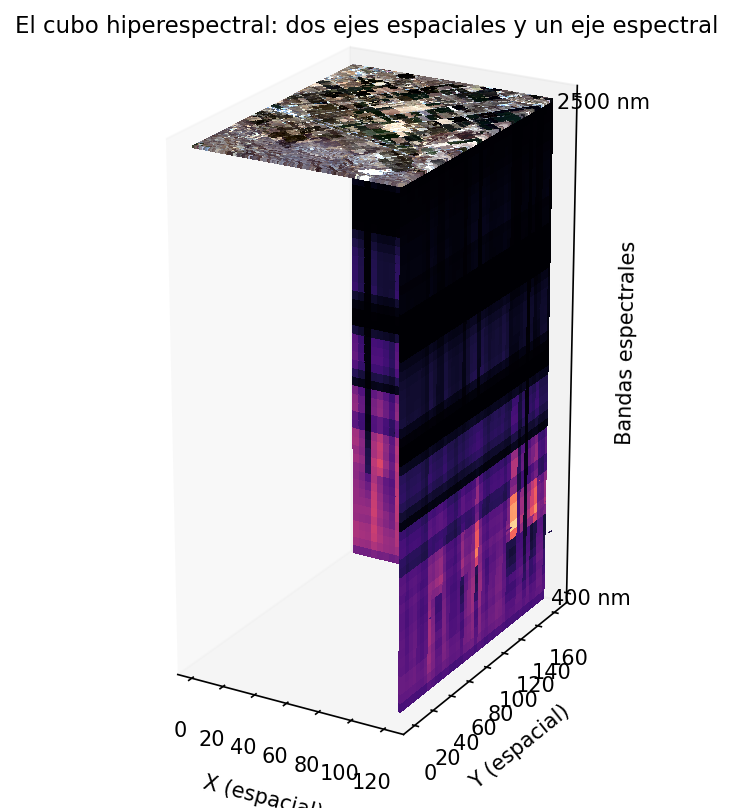
\includegraphics[width=0.62\linewidth]{figuras/hipercubo.png}
\caption{Representación del cubo hiperespectral: dos dimensiones espaciales y una dimensión espectral. La cara superior corresponde a la escena y las caras laterales muestran la variación a lo largo de las bandas.}
\label{fig:hipercubo}
\end{figure}

\begin{figure}[htbp]
\centering
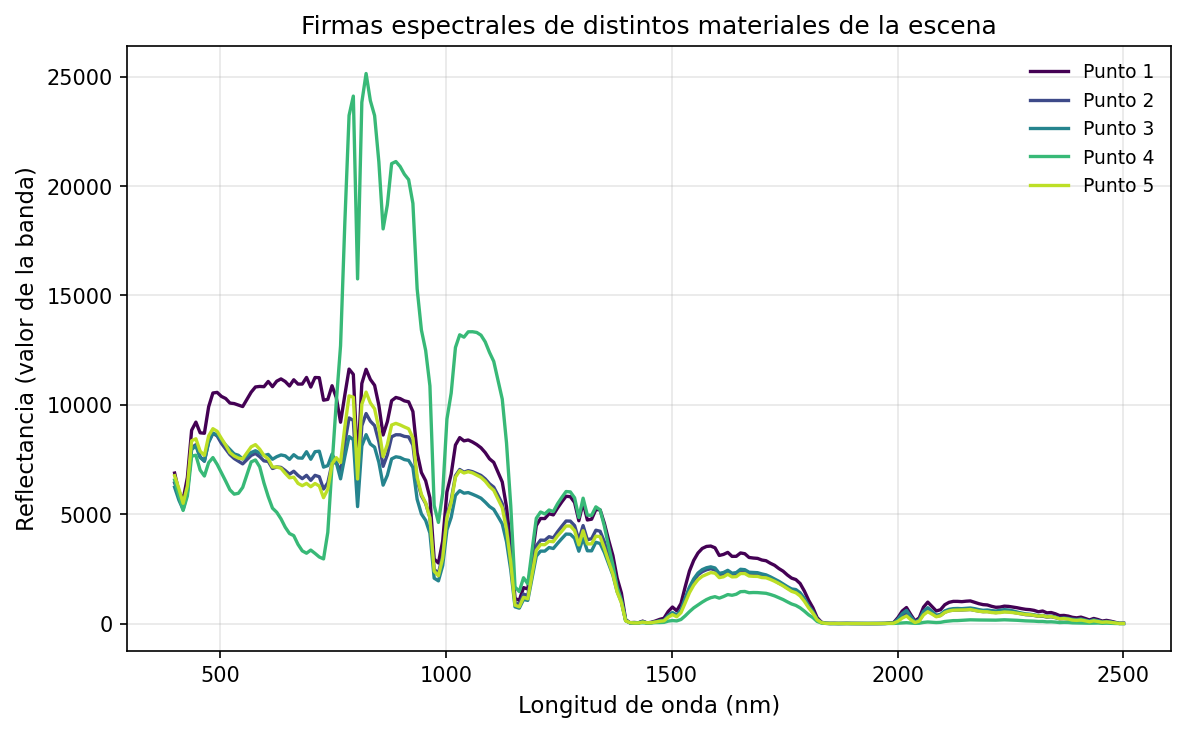
\includegraphics[width=0.85\linewidth]{figuras/firmas_espectrales.png}
\caption{Firmas espectrales de distintos puntos de la escena de prueba. Cada material describe una curva propia de reflectancia frente a la longitud de onda; el punto sobre vegetación muestra el característico salto en el infrarrojo cercano.}
\label{fig:firmas}
\end{figure}

\subsubsection{Detección de cambios bitemporal}
La detección de cambios consiste en comparar dos o más imágenes del mismo lugar capturadas en momentos distintos para identificar las regiones donde se produjo una modificación. En teledetección es una tarea central para el monitoreo del territorio, la evaluación de desastres y el seguimiento del uso del suelo. Actualmente existen técnicas basadas en aprendizaje profundo, que permiten aprender representaciones que capturan información semántica y dan mejores resultados frente a variaciones de iluminación y registro, en lugar de operar simplemente sobre diferencias de píxeles e índices espectrales, que se pueden ver afectados por múltiples factores \cite{khelifi2020deep}. En este trabajo se usarán imágenes hiperespectrales para hacer detección de cambios bitemporal, por lo que se emplearán imágenes de la misma escena en tiempos diferentes.

\begin{figure}[htbp]
\centering
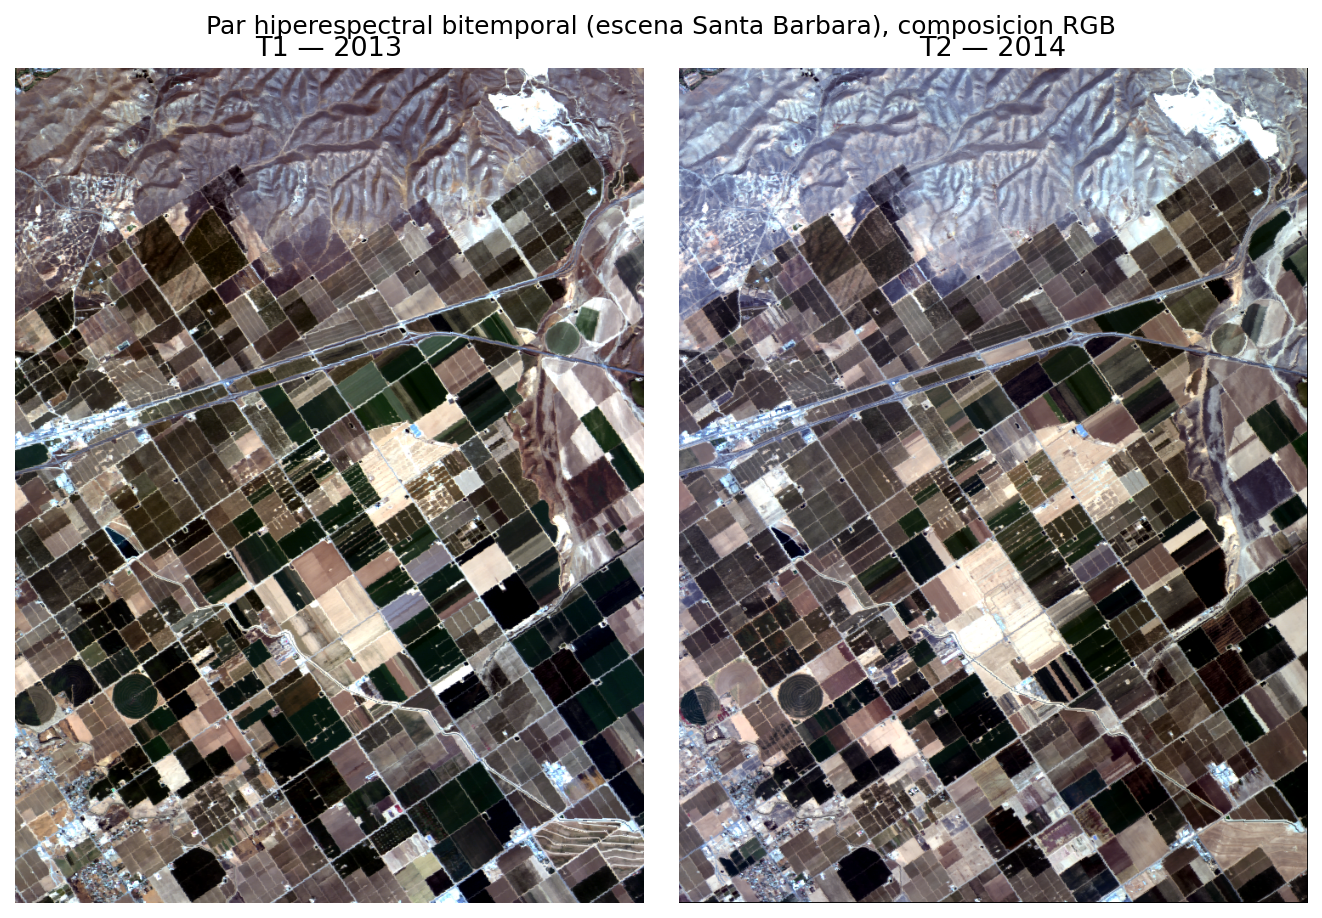
\includegraphics[width=\linewidth]{figuras/par_bitemporal.png}
\caption{Par hiperespectral bitemporal de la misma escena en dos fechas, mostrado como composición RGB. La detección de cambios busca las regiones que difieren entre T1 y T2.}
\label{fig:bitemporal}
\end{figure}

\subsubsection{Segmentación de imágenes}
La segmentación es la tarea de asignar a cada píxel de una imagen una etiqueta que lo agrupa en una región coherente, delimitando objetos o zonas con precisión a nivel de píxel. A diferencia de la clasificación, que asigna una única categoría a toda la imagen, la segmentación produce máscaras que separan cada elemento de la escena.

En cuanto a los modelos que existen, el enfoque tradicional se apoyó en redes convolucionales de tipo codificador y decodificador, como U-Net, Mask R-CNN o DeepLab, que se entrenan de forma supervisada para un conjunto fijo de clases y un dominio concreto. El paradigma actual son los modelos fundacionales de segmentación promptable, cuyo referente es Segment Anything, entrenado sobre un conjunto de datos masivo y capaz de generar máscaras precisas a partir de indicaciones espaciales como puntos o recuadros, sin necesidad de reentrenarse para cada dominio \cite{kirillov2023sam}. Modelos posteriores como SAM 2 extienden esta idea a video, pero comparten el mismo principio de segmentación guiada por indicaciones \cite{ravi2024sam2}.

La aplicación de estos modelos a una imagen hiperespectral no es directa. Segment Anything está diseñado para imágenes naturales de tres canales y no puede recibir como entrada un cubo hiperespectral de cientos de bandas, por lo que se requiere proyectar toda esa información adicional a las tres bandas que puede procesar.

\subsubsection{Transformers y Vision Transformers}
El transformador es una arquitectura de red neuronal basada por completo en el mecanismo de atención, que en lugar de procesar la información de forma local, como hace una convolución, pondera de manera explícita la relación entre todos los elementos de una secuencia y aprende cuáles son relevantes entre sí \cite{vaswani2017attention}. El Vision Transformer traslada esta idea a las imágenes: divide la imagen en parches de tamaño fijo, proyecta cada parche a un vector, los trata como una secuencia de fichas y aplica atención sobre ellos. Su ventaja frente a las redes convolucionales se manifiesta al preentrenarse con grandes volúmenes de datos, régimen en el que aprende representaciones muy transferibles, y por eso se ha convertido en la arquitectura base de los modelos fundacionales de visión \cite{dosovitskiy2021vit}.

Formalmente, la atención de producto punto escalado calcula, a partir de las matrices de consultas $Q$, claves $K$ y valores $V$,
\begin{equation}
\operatorname{Attention}(Q,K,V)=\operatorname{softmax}\!\left(\frac{QK^{\top}}{\sqrt{d_k}}\right)V,
\end{equation}
donde $d_k$ es la dimensión de las claves y el factor $\sqrt{d_k}$ evita que el producto crezca demasiado y sature la función softmax. Cada elemento de la secuencia queda así representado como una combinación ponderada de los demás, con pesos que expresan su relevancia mutua \cite{vaswani2017attention}.

\subsubsection{Modelos fundacionales}
Un modelo fundacional es un modelo de gran escala preentrenado sobre cantidades masivas de datos, diseñado para servir como base reutilizable en múltiples tareas posteriores sin necesidad de entrenarlo desde cero. Para imágenes hiperespectrales, HyperSIGMA es el primer modelo fundacional con más de mil millones de parámetros, preentrenado sobre un conjunto extenso de imágenes, capaz de extraer características espaciales y espectrales transferibles a tareas como clasificación, detección de cambios y segmentación \cite{wang2024hypersigma}. Esto permite aprovechar su gran capacidad de generalización, así como la posibilidad de usar modelos ya entrenados con más datos de los que normalmente se tendrían disponibles; entrenar uno desde cero sería una tarea muy difícil y posiblemente daría resultados inferiores debido a las limitaciones de datos de entrenamiento y de equipo necesario.

En los últimos años, los modelos fundacionales se han convertido en una herramienta central de la investigación en visión por computadora y teledetección. Su capacidad de transferir el conocimiento adquirido en el preentrenamiento a tareas nuevas, con pocos o ningún ejemplo etiquetado, ha impulsado su adopción en problemas donde los datos anotados son escasos o costosos, como ocurre con las imágenes hiperespectrales. Esta tendencia se refleja en la aparición de modelos fundacionales propios del dominio \cite{wang2024hypersigma}, en enfoques de clasificación sin entrenamiento específico \cite{pang2025special} y en la detección de cambios semánticos apoyada en estos modelos \cite{zhu2025semanticcd}.

\subsubsection{Arquitectura de HyperSIGMA: SpatViT y atención por muestreo disperso}
La extracción de características de este trabajo recae en SpatViT, la subred espacial de HyperSIGMA. Es un Vision Transformer que divide la imagen hiperespectral en parches no solapados y los procesa con atención; en la variante base que se emplea aquí, produce un mapa de características denso de dimensión de \textit{embedding} 768 a un dieciseisavo de la resolución espacial de entrada \cite{wang2024hypersigma}.

El problema es que la autoatención completa tiene un costo cuadrático en el número de fichas, y las imágenes hiperespectrales presentan una fuerte redundancia espacial y espectral, por lo que atender de forma uniforme a todas las posiciones es ineficiente. SpatViT lo resuelve con la atención por muestreo disperso. En lugar de comparar cada consulta con todas las claves, cada consulta $\mathbf{q}$ predice $N_p$ desplazamientos de muestreo mediante una proyección lineal aprendida $W_p$, y las claves y los valores se muestrean únicamente en esas posiciones desplazadas mediante interpolación bilineal, formando los conjuntos reducidos $K'$ y $V'$. La atención se calcula entonces solo sobre ese conjunto disperso:
\begin{equation}
\operatorname{SSA}(Q,K',V')=\operatorname{softmax}\!\left(\frac{Q\,K'^{\top}}{\sqrt{D'}}\right)V',
\end{equation}
donde $D'$ es la dimensión de las claves. Así, cada consulta aprende qué regiones son relevantes en vez de recorrerlas todas, lo que captura contexto diverso de largo alcance con un costo mucho menor que la autoatención completa \cite{wang2024hypersigma}. En el pipeline, SpatViT con esta atención es el codificador que genera las representaciones de la imagen inicial y la final, sobre las que se calcula el mapa de cambio por similitud coseno.

\subsubsection{Aprendizaje zero-shot}
El aprendizaje zero-shot se refiere a la capacidad de un modelo para resolver una tarea o reconocer categorías que no aparecieron durante su entrenamiento, apoyándose en el conocimiento general adquirido en el preentrenamiento. Modelos como CLIP usan esta técnica para clasificar imágenes en categorías descritas únicamente mediante texto, sin haber visto ejemplos etiquetados de esas categorías \cite{radford2021clip}. En el ámbito hiperespectral, trabajos recientes llevan esta idea a la clasificación de coberturas del suelo, o \textit{land covers}, sin entrenamiento específico \cite{pang2025special}. El sistema propuesto es zero-shot en tanto no requiere entrenar sobre pares de imágenes hiperespectrales etiquetados para detectar y nombrar los cambios. Esto está alineado con el uso de modelos fundacionales, ya que el enfoque permite aprovechar todas sus ventajas sin tener que entrenar necesariamente un modelo propio.

\subsubsection{Vocabulario abierto}
El enfoque de vocabulario abierto permite etiquetar regiones de una imagen con cualquier concepto expresable en lenguaje natural, en lugar de restringirse a un conjunto cerrado y predefinido de clases. Un clasificador clásico se entrena sobre un número fijo de categorías, por ejemplo agua, vegetación o edificación, y solo puede responder con una de esas etiquetas aprendidas. Si aparece un concepto nuevo que no estaba en ese conjunto, el modelo no puede nombrarlo, y para agregarlo hay que anotar datos nuevos y volver a entrenar la red por completo, por lo cual no es muy práctico.

El vocabulario abierto funciona de otra forma y soluciona el problema. En lugar de una capa final con un número fijo de salidas, se emplean modelos que proyectan imágenes y texto a un mismo espacio de representación, de tal modo que la etiqueta se decide comparando la región con la descripción textual de cada categoría candidata \cite{radford2021clip}. Las categorías ya no son fijas en la red, sino que se entregan como texto en el momento de la consulta, y pueden cambiarse o ampliarse sin reentrenar nada \cite{kombol2025trainingfree}.

El vocabulario tradicional funciona como una especie de formulario en donde solo se puede elegir entre opciones predeterminadas, mientras que el vocabulario abierto funciona más como un prompt, en donde se escribe con lenguaje natural y el modelo decide cuál opción encaja mejor con la imagen.

\subsubsection{Modelos de visión-lenguaje y descripción de imágenes}
Los modelos de visión-lenguaje aprenden una representación conjunta de imágenes y texto a partir de grandes colecciones de pares imagen y descripción, con el fin de resolver tareas visuales guiadas por lenguaje sin entrenar un modelo distinto para cada una \cite{zhang2024vlm}. CLIP es el exponente que se emplea en este trabajo: entrena dos codificadores, uno visual y uno textual, para proyectar ambas modalidades a un espacio común donde la correspondencia se mide por similitud, lo que habilita la clasificación por texto libre y el etiquetado de vocabulario abierto \cite{radford2021clip}.

La descripción de imágenes, también llamada generación de subtítulos, va un paso más allá de la clasificación: en vez de asignar una etiqueta, genera una frase en lenguaje natural que resume el contenido visual. Los primeros modelos neuronales de esta tarea se dividen en dos fases, un codificador convolucional que condensa la imagen en un vector y un decodificador recurrente que, a partir de ese vector, produce la frase palabra por palabra; sus autores lo describen como un modelo que ``se puede usar para generar frases naturales que describen una imagen'' \cite{vinyals2015show}. Hoy la línea la dominan los modelos de visión-lenguaje preentrenados a gran escala, como BLIP, que reúnen en una sola arquitectura la comprensión de la imagen y la generación del texto que la describe \cite{li2022blip}.

En teledetección, la descripción de imágenes se apoya en conjuntos de datos propios. RSICD, por ejemplo, reúne cerca de once mil imágenes de teledetección con varias descripciones cada una, y permite entrenar y evaluar modelos adaptados a las escenas aéreas y satelitales \cite{lu2017rsicd}. Esos avances se dieron sobre imágenes ópticas de tres canales y no hiperespectrales. La extensión al dominio hiperespectral llegó con HyperCap, el primer punto de referencia para describir coberturas de terreno a partir de imágenes hiperespectrales, que hace posible aplicar modelos de visión-lenguaje sobre el cubo espectral completo \cite{das2025hypercap}.

En el sistema, estos modelos ocupan las dos últimas etapas semánticas del pipeline. CLIP asigna a cada región de cambio una etiqueta de vocabulario abierto por similitud entre imagen y texto \cite{radford2021clip}, y un modelo de descripción de tipo BLIP, adaptado sobre HyperCap, genera una frase en lenguaje natural que caracteriza la región con más riqueza que una sola etiqueta \cite{li2022blip,das2025hypercap}.

\subsubsection{Representaciones vectoriales y similitud coseno}
El aprendizaje profundo parte de que el desempeño en una tarea depende sobre todo de la calidad de la representación de los datos \cite{bengio2013representation}. Un modelo profundo transforma cada imagen o región en un vector de características o \textit{embedding} $\mathbf{v}\in\mathbb{R}^{d}$, con $d$ del orden de cientos, en un espacio donde la proximidad entre vectores corresponde a similitud semántica.

La comparación entre dos \textit{embeddings} $\mathbf{u}$ y $\mathbf{v}$ usa la similitud coseno:
\begin{equation}
\operatorname{sim}(\mathbf{u},\mathbf{v})=\frac{\mathbf{u}\cdot\mathbf{v}}{\lVert\mathbf{u}\rVert\,\lVert\mathbf{v}\rVert}=\frac{\sum_{i=1}^{d}u_i v_i}{\sqrt{\sum_{i=1}^{d}u_i^{2}}\,\sqrt{\sum_{i=1}^{d}v_i^{2}}}\in[-1,1].
\end{equation}
La normalización por las magnitudes $\lVert\mathbf{u}\rVert$ y $\lVert\mathbf{v}\rVert$ elimina la escala y conserva solo la orientación, por lo que la medida es insensible a diferencias de brillo o ganancia entre las dos capturas.

HyperSIGMA entrega un \textit{embedding} por posición del mapa de características \cite{wang2024hypersigma}. Para cada posición $p$, con vectores $\mathbf{e}_1(p)$ y $\mathbf{e}_2(p)$ de las imágenes inicial y final, el mapa de cambio es
\begin{equation}
C(p)=1-\operatorname{sim}\!\big(\mathbf{e}_1(p),\mathbf{e}_2(p)\big),
\end{equation}
donde un valor alto indica cambio y uno bajo permanencia. En la implementación $C$ se interpola de forma bilineal al tamaño original, se renormaliza a $[0,1]$ y se binariza con el método de Otsu para delimitar las regiones de cambio. La misma similitud coseno rige el etiquetado, al comparar el \textit{embedding} de una región con el de cada descripción textual candidata.

\subsubsection{Métricas de evaluación}
La evaluación de la detección de cambios se plantea como una comparación píxel a píxel entre el resultado del sistema y una verdad de terreno, de la que surgen cuatro conteos: verdaderos positivos $VP$ cuando se detecta un cambio real, verdaderos negativos $VN$ cuando se identifica correctamente una zona sin cambio, falsos positivos $FP$ cuando se señala un cambio inexistente y falsos negativos $FN$ cuando se pasa por alto un cambio real. Sobre estos conteos se definen las métricas de desempeño.

La precisión $P$ mide qué proporción de los cambios detectados son correctos y penaliza los falsos positivos, mientras que la exhaustividad $R$ mide qué proporción de los cambios reales se detectaron y penaliza los falsos negativos:
\begin{equation}
P=\frac{VP}{VP+FP},\qquad R=\frac{VP}{VP+FN}.
\end{equation}
Como suele existir una tensión entre ambas, el puntaje F1 las combina en un único valor mediante su media armónica, que solo es alta cuando las dos lo son:
\begin{equation}
F_1=\frac{2\,P\,R}{P+R}=\frac{2\,VP}{2\,VP+FP+FN}.
\end{equation}
La intersección sobre unión evalúa el solapamiento espacial entre la región detectada y la real, dividiendo el área común entre el área total que cubren juntas:
\begin{equation}
\mathrm{IoU}=\frac{VP}{VP+FP+FN}.
\end{equation}
Estas métricas son el estándar en la revisión de métodos de detección de cambios basados en aprendizaje profundo \cite{khelifi2020deep}. En este trabajo son la base de la validación cuantitativa del sistema: la máscara de cambio producida por el pipeline se contrasta con la verdad de terreno de un conjunto hiperespectral bitemporal de referencia, y los valores de precisión, exhaustividad y puntaje F1 permiten situar el desempeño frente a métodos existentes.

\subsubsection{Modelos y datos empleados en el sistema}
Las tres piezas centrales del pipeline comparten el mismo esqueleto arquitectónico, el Vision Transformer. En la extracción de características, HyperSIGMA procesa cada imagen con un codificador de tipo Vision Transformer espacial, en su variante base, que divide el cubo en parches y produce mapas de características densos a partir de los cuales se calcula el mapa de cambio \cite{wang2024hypersigma}. En la segmentación, Segment Anything delimita las regiones con un codificador de imagen Vision Transformer de gran tamaño \cite{kirillov2023sam}. Y en el etiquetado, CLIP asigna las etiquetas de vocabulario abierto mediante un codificador visual Vision Transformer alineado con el texto \cite{radford2021clip}. Así, el mismo principio de atención sobre parches recorre la detección de características, la segmentación y el etiquetado, lo que da coherencia arquitectónica a todo el sistema.

A continuación se reúnen, ya como tecnología concreta, las piezas del sistema:
\begin{itemize}
    \item \textbf{HyperSIGMA} --- modelo fundacional hiperespectral basado en Vision Transformer, escalable a más de mil millones de parámetros y preentrenado sobre un conjunto masivo de imágenes hiperespectrales. Extrae las representaciones profundas de cada imagen, sobre las que se calcula el mapa de cambio \cite{wang2024hypersigma}.
    \item \textbf{Segment Anything} --- modelo fundacional de segmentación promptable con codificador Vision Transformer de gran tamaño. Convierte las regiones de cambio en máscaras precisas a nivel de píxel a partir de indicaciones espaciales \cite{kirillov2023sam}.
    \item \textbf{CLIP} --- modelo de visión-lenguaje que alinea imagen y texto en un espacio común. Asigna a cada región una etiqueta de vocabulario abierto por similitud entre la imagen y las descripciones textuales candidatas \cite{radford2021clip}.
    \item \textbf{BLIP} --- modelo de visión-lenguaje que unifica comprensión y generación. Genera la descripción en lenguaje natural de cada región, adaptado sobre datos hiperespectrales \cite{li2022blip}.
    \item \textbf{HyperCap} --- primer conjunto de datos y punto de referencia para la descripción de imágenes hiperespectrales, con anotaciones textuales a nivel de píxel. Sirve de base de entrenamiento y evaluación del módulo de descripción \cite{das2025hypercap}.
\end{itemize}

\subsection{Estado del arte}
El estado del arte se organiza siguiendo el recorrido del pipeline. Para cada etapa se revisa cómo se resuelve hoy el problema, qué alternativas existen, y se justifica la herramienta elegida; al mencionar cada modelo se indica quién lo desarrolla. El sistema no propone modelos nuevos, sino que integra modelos fundacionales de referencia, cada uno líder en su tarea.

\subsubsection{Imágenes hiperespectrales y su adquisición}
La imagen hiperespectral nace de la espectrometría de imagen, formulada por Goetz en 1985 como la adquisición simultánea de imágenes en muchas bandas espectrales contiguas para obtener, en cada píxel, un espectro completo con el que identificar los materiales de la superficie terrestre \cite{goetz1985imaging}. La tecnología ha evolucionado en gran medida desde los primeros sensores aerotransportados, como AVIRIS del Jet Propulsion Laboratory de la NASA, hacia sensores satelitales como Hyperion del satélite EO-1, que amplían el rango de cobertura y permiten disponer de más datos con cientos de bandas \cite{bhargava2024hyperspectral}.

Para la adquisición existen dos métodos que son los más usados: los sensores de empuje, o pushbroom, que registran una línea espacial completa en todas las bandas a la vez, y los de barrido por punto, o whiskbroom, que recorren la escena punto a punto. Existen también cámaras instantáneas que capturan todo el cubo a la vez, pero pierden resolución frente a las otras alternativas; siempre hay una relación de compromiso entre resolución espacial, resolución espectral y relación señal a ruido, y hay que decidir qué característica se prioriza frente a las demás. En este trabajo los datos entran como pares bitemporales en formatos ENVI, MATLAB o GeoTIFF, y se reinterpolan a un espacio espectral de referencia, el del sensor Hyperion, que es el mismo con el que se preentrena el modelo fundacional que extrae las características.

\subsubsection{Extracción de características: transformers y modelos fundacionales hiperespectrales}
La tecnología clave en todos los modelos fundacionales usados en el proyecto son los transformers, propuestos por Vaswani, de Google, en 2017, que sustituyen la convolución y la recurrencia por el mecanismo de atención \cite{vaswani2017attention}. En 2021 la tecnología se adaptó a las imágenes con el Vision Transformer de Dosovitskiy, de Google, que trata la imagen como una secuencia de parches \cite{dosovitskiy2021vit}. A partir de esto surgen los modelos fundacionales, preentrenados a gran escala y reutilizables sin tener que entrenar desde cero.

Para obtener la representación de la imagen hiperespectral hay dos formas principales. La tradicional es calcularla a mano mediante índices espectrales, fórmulas que combinan bandas concretas para resaltar un material; el problema es que para saber qué fórmula usar y de qué modo se necesita saber de antemano qué se quiere resaltar. La alternativa moderna, que adopta este trabajo, es aprenderla con un modelo fundacional. HyperSIGMA representa la imagen dividiendo el cubo en parches y procesándolos con un Vision Transformer espacial que, mediante su atención por muestreo disperso, produce un mapa denso de vectores de características, uno por posición, que codifican de forma conjunta la información espacial y espectral de la escena. Es el primer modelo fundacional hiperespectral con más de mil millones de parámetros, desarrollado por Wang, de la Universidad de Wuhan, y preentrenado sobre el conjunto HyperGlobal-450K con cerca de 450.000 imágenes \cite{wang2024hypersigma}. La elección se justifica porque estas representaciones son de mejor calidad que las de un índice manual y, al haberse aprendido sobre datos hiperespectrales, resultan transferibles a tareas nuevas sin reentrenar. El código es público en el repositorio oficial del grupo WHU-Sigma \cite{whu2024hypersigma_repo}.

\begin{figure}[htbp]
\centering
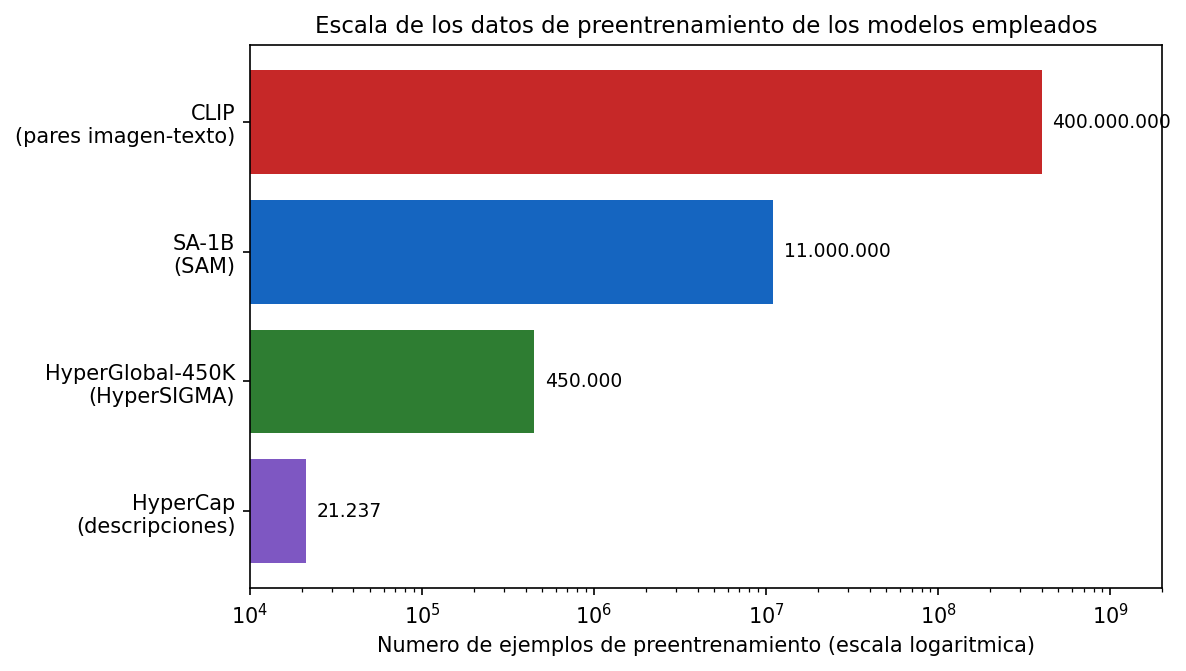
\includegraphics[width=0.85\linewidth]{figuras/benchmark.png}
\caption{Escala de los datos de preentrenamiento de los modelos fundacionales empleados, en escala logarítmica. Las cifras provienen de las publicaciones de cada modelo; nótese que las unidades difieren entre imágenes, pares imagen-texto y descripciones.}
\label{fig:benchmark}
\end{figure}

\subsubsection{Detección de cambios y el emparejamiento en el espacio latente}
Las técnicas se agrupan en cuatro grupos. Las de álgebra de imágenes trabajan directamente sobre los valores de los píxeles, como la diferencia, el cociente o el análisis de vectores de cambio. Las de transformación proyectan los datos a otro espacio antes de compararlos para que la información útil quede más concentrada y fácil de leer, por ejemplo usando PCA. Las de comparación post-clasificación clasifican cada imagen por separado y luego contrastan las clases. Y, de forma dominante hoy, las de aprendizaje profundo aprenden a detectar el cambio con redes siamesas y de atención \cite{khelifi2020deep}. En cuanto a en qué se aplica, la detección de cambios opera sobre imágenes multiespectrales, de radar de apertura sintética y, cada vez más, hiperespectrales, donde la alta resolución espectral permite detectar cambios pequeños; un ejemplo es GETNET, una red convolucional de dos dimensiones de extremo a extremo propuesta por Wang en 2019 para detección de cambios hiperespectral \cite{wang2019getnet}. Esta funciona usando información de abundancia a nivel de subpíxel obtenida por desmezclado espectral y la combina en una matriz de afinidad mixta que fusiona varias fuentes de información; sobre esa representación, la red aprende a clasificar cada píxel como cambiado o no cambiado, y así maneja más fácilmente la alta dimensionalidad del cubo. Los autores también publicaron un conjunto de datos llamado River, cuyo objetivo es probar los distintos métodos y comparar cuál funciona mejor sobre los mismos datos.

La mayoría de estos métodos requiere entrenar con pares etiquetados, escasos en el dominio hiperespectral. La alternativa que adopta este trabajo es saltar el entrenamiento: se comparan las representaciones que HyperSIGMA extrae de las dos capturas mediante la similitud coseno, emparejando vectores en un espacio latente común; cuando la similitud entre las representaciones inicial y final es baja, se toma como que hay cambio. Esta es la misma métrica que usan modelos como CLIP \cite{radford2021clip}. La técnica se justifica por ser un enfoque zero-shot, que no depende de datos etiquetados de cambio y aprovecha directamente la calidad de las representaciones del modelo fundacional.

\subsubsection{Segmentación}
La segmentación es una parte fundamental del sistema. Su estado del arte pasa de las redes convolucionales de codificador y decodificador, como U-Net de Ronneberger en 2015 \cite{ronneberger2015unet}, Mask R-CNN de He, de Facebook AI Research, en 2017 \cite{he2017maskrcnn} y la familia DeepLab, todas entrenadas para un conjunto fijo de clases, al paradigma de los modelos fundacionales de segmentación promptable. El referente es Segment Anything, desarrollado por Meta AI en 2023, entrenado sobre el conjunto SA-1B con once millones de imágenes y mil millones de máscaras, capaz de segmentar cualquier objeto a partir de indicaciones espaciales sin reentrenarse \cite{kirillov2023sam}; su sucesor, SAM 2, tiene la misma capacidad pero en video \cite{ravi2024sam2}. El modelo y sus pesos están disponibles en el sitio oficial de Meta \cite{meta2023sam_repo}.

Las alternativas entrenadas por clase exigirían anotar datos de las coberturas de interés, lo que no aborda la característica de vocabulario abierto del problema. Por esta razón, se propone usar Segment Anything, porque produce máscaras precisas sin depender de clases predefinidas ni de reentrenamiento, y se integra de forma natural recibiendo como indicaciones los puntos y recuadros derivados del mapa de cambio. Como opera sobre imágenes de tres canales, se le entrega una composición RGB del cubo hiperespectral, y cada máscara se confina a la región de cambio.

\subsubsection{Etiquetado de vocabulario abierto}
Para nombrar cada región sin un conjunto cerrado de clases, se usan modelos de visión-lenguaje, que alinean imagen y texto en un espacio común \cite{zhang2024vlm}. El referente es CLIP, desarrollado por OpenAI en 2021, entrenado por contraste sobre cerca de cuatrocientos millones de pares imagen-texto, que clasifica en modo zero-shot comparando la imagen con descripciones textuales arbitrarias \cite{radford2021clip}; su implementación oficial es pública \cite{openai2021clip_repo}. En teledetección esta idea ya se traslada a la segmentación y la detección de cambios de vocabulario abierto \cite{kombol2025trainingfree,zhu2025semanticcd}, y en el dominio hiperespectral a la clasificación zero-shot \cite{pang2025special}.

La alternativa tradicional, un clasificador de clases fijas, obligaría a definir de antemano todo lo que puede aparecer y a reentrenar para añadir una categoría. Este trabajo usa CLIP porque convierte el etiquetado en una comparación por similitud contra un vocabulario de texto libre, editable sin reentrenar, que es la esencia del objetivo de vocabulario abierto. En el pipeline, CLIP asigna a cada máscara la etiqueta más afín de ese vocabulario.

\subsubsection{Descripción en lenguaje natural}
La última etapa amplía la etiqueta con una frase en lenguaje natural, de modo que el prompt y la etiqueta coincidan, funcionando esta etapa como una especie de traductor. La descripción de imágenes nace con modelos de codificador convolucional y decodificador recurrente, como Show and Tell de Vinyals, de Google, en 2015 \cite{vinyals2015show}, y hoy la dominan los modelos de visión-lenguaje preentrenados como BLIP, desarrollado por Salesforce Research en 2022, que unifica comprensión y generación \cite{li2022blip}; su código es público \cite{salesforce2022blip_repo}. En teledetección la descripción cuenta con conjuntos propios como RSICD \cite{lu2017rsicd}, pero limitados a imágenes ópticas de tres canales. El salto al dominio hiperespectral es muy reciente y lo habilita HyperCap, el primer conjunto de descripción hiperespectral con anotaciones a nivel de píxel, desarrollado por Das, del Vellore Institute of Technology \cite{das2025hypercap}.

La alternativa de aplicar un modelo de descripción de imágenes naturales ignora la información espectral del cubo. Por eso este trabajo, en su etapa opcional de descripción, adapta un modelo de tipo BLIP cuyo codificador visual se sustituye por uno que consume directamente el cubo hiperespectral, entrenado sobre HyperCap. Se justifica porque genera una caracterización más rica que una sola etiqueta y aprovecha la dimensión espectral completa.

\subsubsection{Aprendizaje zero-shot}
El aprendizaje zero-shot designa la capacidad de un modelo para resolver una tarea o reconocer categorías que no aparecieron en su entrenamiento, basándose en conocimiento previo que relaciona lo conocido con lo nuevo. El término aparece con Palatucci en 2009, que predice clases nunca vistas mediante códigos de salida semánticos \cite{palatucci2009zeroshot}, en paralelo con los enfoques basados en atributos de Lampert, que transfieren descripciones entre clases \cite{lampert2009attribute}.

Con el tiempo empiezan a surgir los modelos preentrenados a gran escala y el zero-shot se consolida como una técnica ampliamente utilizada; un ejemplo es CLIP, que clasifica imágenes en categorías descritas solo con texto, sin ejemplos etiquetados \cite{radford2021clip}, y la idea se extiende al reconocimiento de vocabulario abierto y la segmentación \cite{kombol2025trainingfree}, a la clasificación hiperespectral en teledetección \cite{pang2025special} y a la detección de cambios semánticos \cite{zhu2025semanticcd}. Su validez descansa en que un modelo fundacional, tras preentrenarse sobre volúmenes masivos de datos, captura conocimiento general y transferible, que permite generalizar a tareas y categorías nuevas sin verlas, siempre que se expresen en un espacio semántico común, por ejemplo el del lenguaje \cite{wang2024hypersigma,radford2021clip}.

Las alternativas son el aprendizaje supervisado, que exige un conjunto etiquetado para cada tarea y clase; el ajuste fino de un modelo preentrenado, que necesita algunos ejemplos anotados; y el aprendizaje con pocos ejemplos, o few-shot. Todas requieren datos etiquetados del problema concreto. Este trabajo adopta el zero-shot porque los pares hiperespectrales bitemporales con verdad de terreno son escasos y difíciles de anotar, ya que el proceso sería manual, y porque el objetivo mismo, detectar y nombrar cambios con vocabulario libre, es incompatible con un conjunto cerrado de clases entrenadas. El sistema utiliza modelos fundacionales sin entrenar sobre la tarea: compara representaciones por similitud coseno para el cambio y compara con texto para la etiqueta, de modo que todo el proceso opera sin ejemplos etiquetados de detección de cambios.

\subsubsection{Vacío de investigación}
El estado del arte muestra que cada pieza está resuelta por separado: hay modelos fundacionales hiperespectrales \cite{wang2024hypersigma}, segmentación promptable \cite{kirillov2023sam}, etiquetado de vocabulario abierto \cite{radford2021clip} y descripción hiperespectral \cite{das2025hypercap}. El vocabulario abierto y el zero-shot están consolidados en imágenes RGB y empiezan a aparecer en teledetección \cite{zhu2025semanticcd,kombol2025trainingfree}. Sin embargo, ninguna propuesta los integra para detectar y describir cambios, con vocabulario libre y sin entrenamiento, sobre imágenes hiperespectrales bitemporales. Ese vacío es el que aborda este trabajo.

    \newpage
% ================= METODOLOGÍA =================
\section{\textbf{Metodología}}
Para el desarrollo de este trabajo se propone una metodología organizada en fases, cada una compuesta por un conjunto de actividades que describen las acciones concretas requeridas para llevarla a cabo. La Figura~\ref{fig:pipeline} resume la cadena de procesamiento del sistema, indicando en cada etapa el modelo empleado; las fases de esta metodología siguen ese mismo recorrido.

\begin{figure}[htbp]
\centering
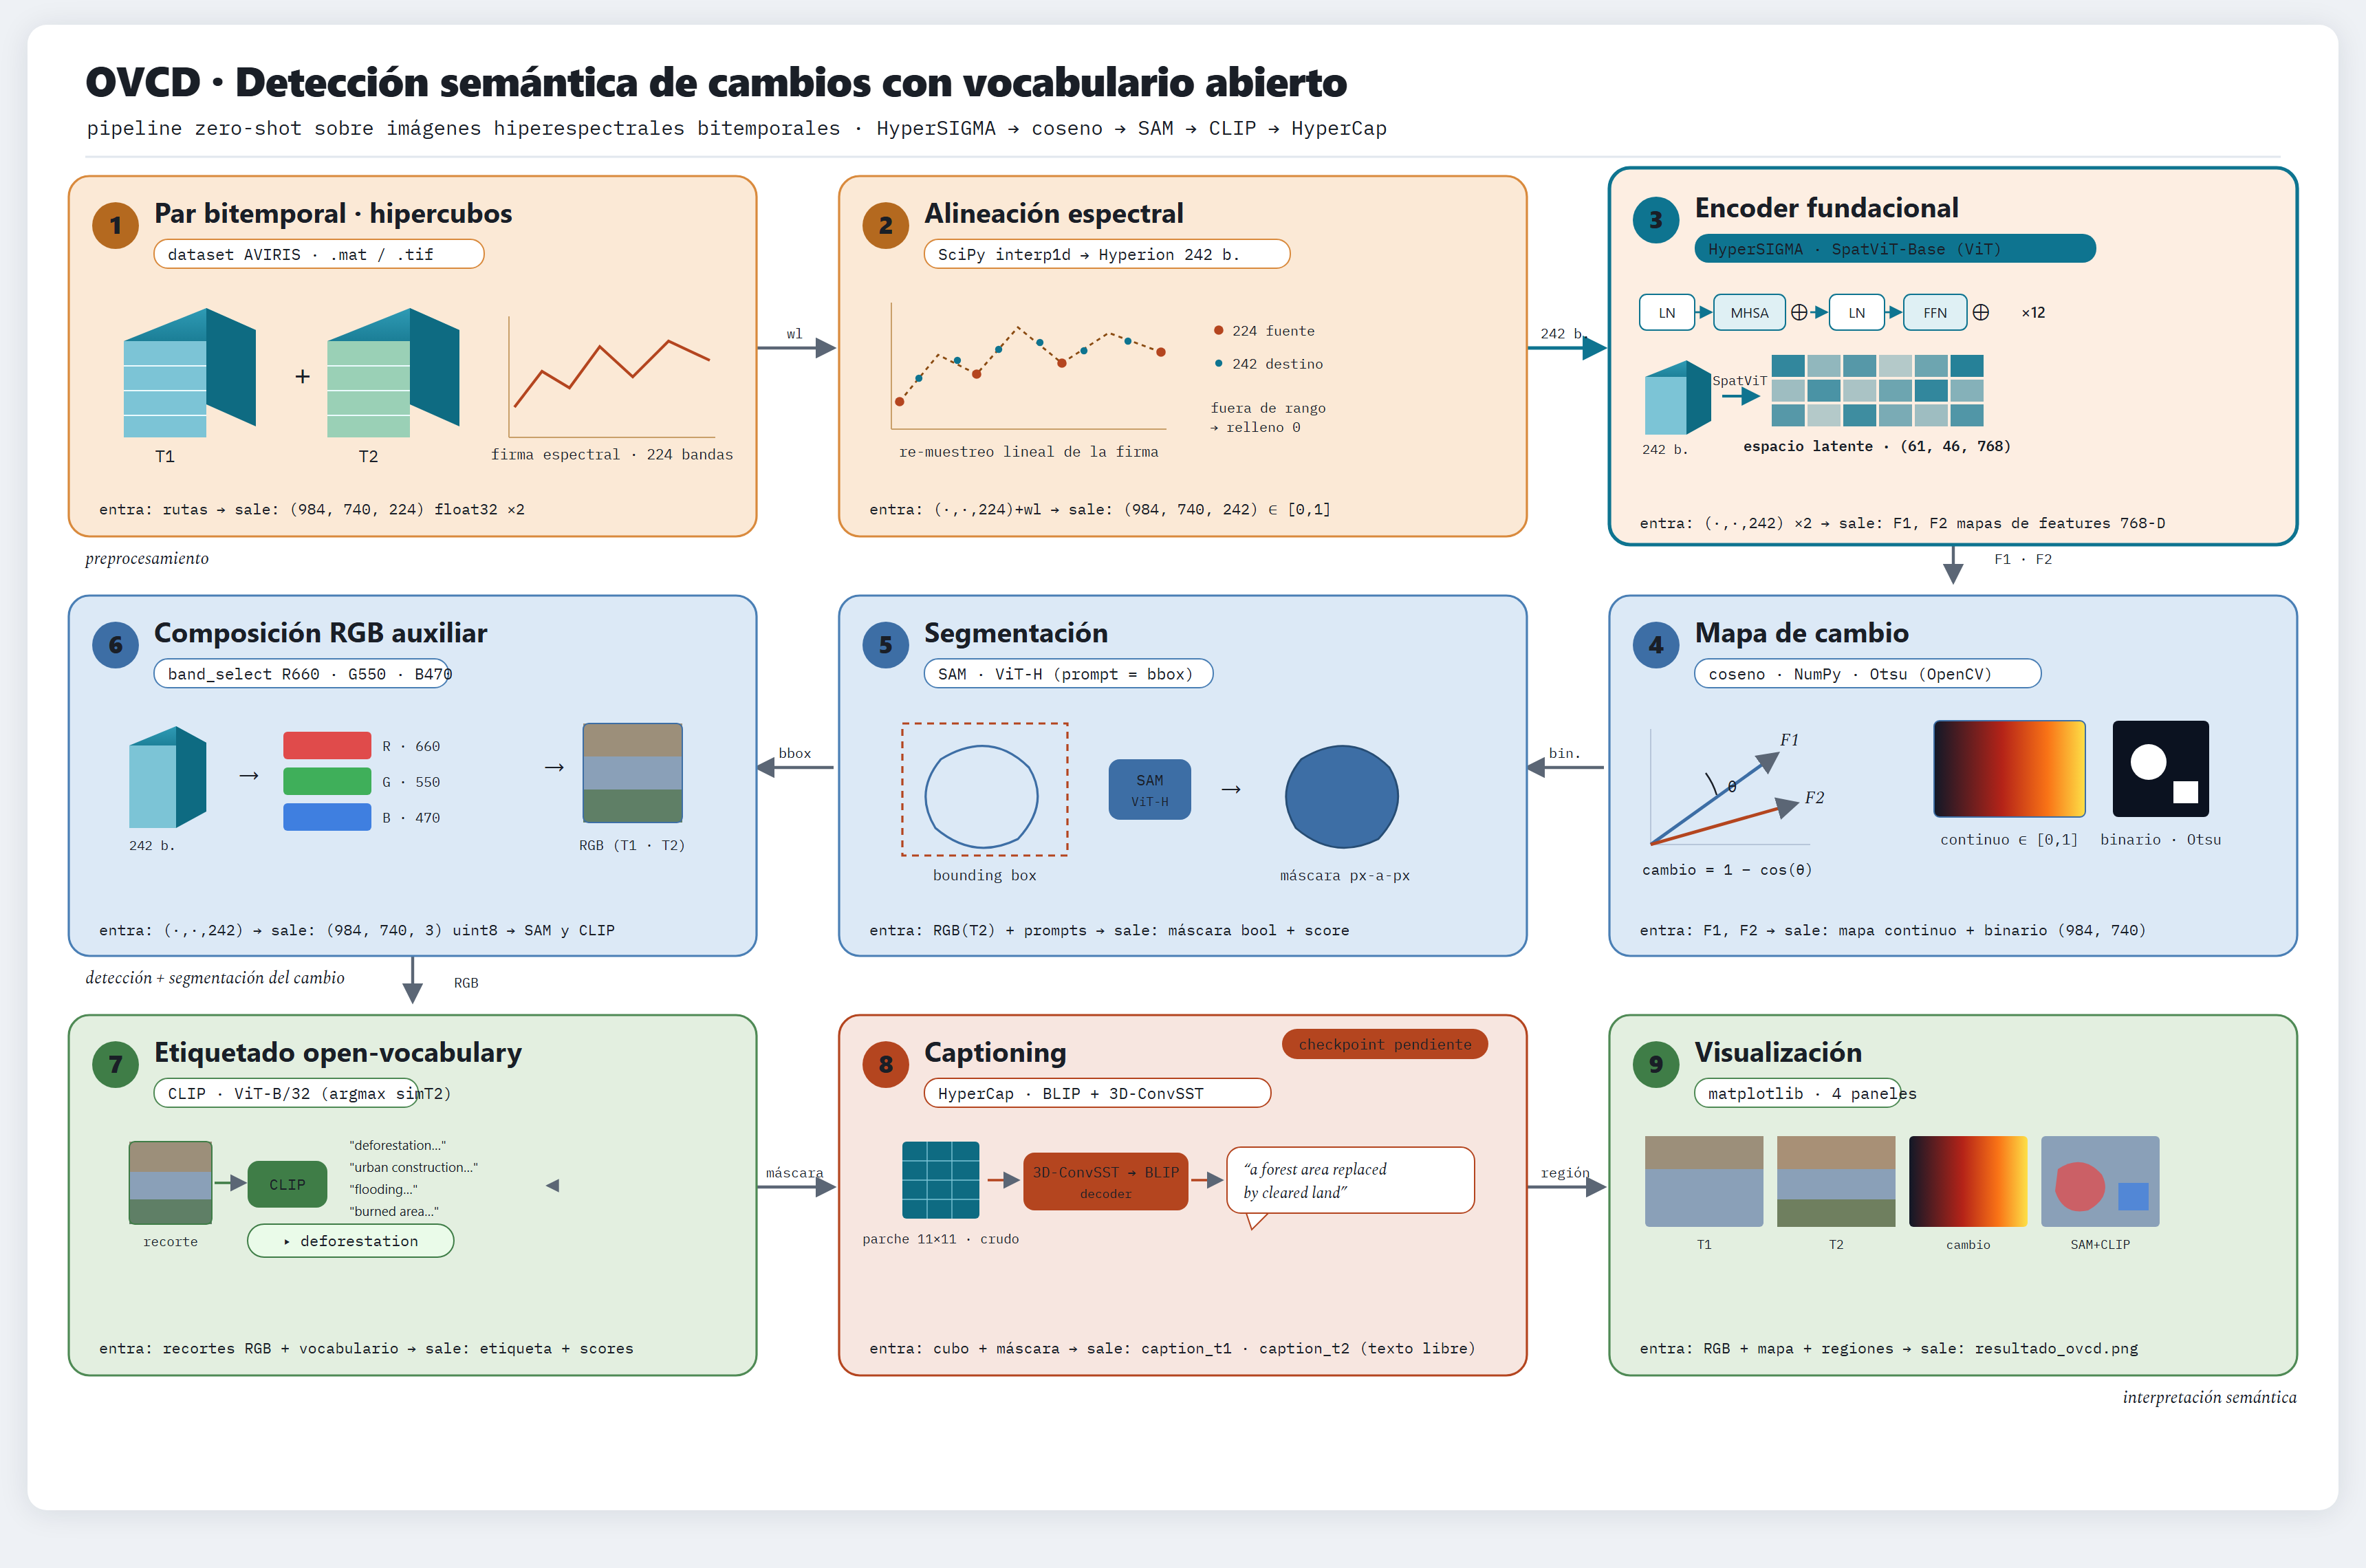
\includegraphics[width=\linewidth]{figuras/pipeline_figura.png}
\caption{Cadena de procesamiento del sistema OVCD, organizada en tres bloques: preprocesamiento, detección y segmentación del cambio, e interpretación semántica. El par bitemporal se carga y se alinea a un espacio espectral común; HyperSIGMA extrae las características de cada imagen; su comparación por similitud coseno produce el mapa de cambio; Segment Anything segmenta las regiones sobre una composición RGB; CLIP les asigna una etiqueta de vocabulario abierto; y, de forma opcional, un modelo de tipo BLIP adaptado sobre HyperCap genera una descripción.}
\label{fig:pipeline}
\end{figure}

\subsection{{Fase 1. Carga y alineación espectral}}

Esta fase comprende la lectura de los pares de imágenes hiperespectrales bitemporales y su preparación para el análisis, de modo que ambas adquisiciones queden expresadas en un mismo espacio espectral y en un rango de valores homogéneo.

\subsubsection{{Actividad 1.1. Carga de los pares hiperespectrales}}

Se implementará un módulo de carga capaz de leer imágenes hiperespectrales en formatos ENVI, MATLAB y GeoTIFF, extrayendo de cada archivo el cubo de datos con sus dimensiones espaciales y espectrales, junto con las longitudes de onda asociadas a cada banda. Cuando el archivo no contenga la información de las bandas, la imagen se descartará, ya que esa información es necesaria para alinear las adquisiciones a un espacio espectral de referencia común.

\subsubsection{{Actividad 1.2. Alineación a un espacio espectral de referencia}}

Se reinterpolarán las bandas de ambas imágenes a un espacio espectral de referencia común mediante interpolación lineal, garantizando que las dos adquisiciones tengan el mismo número de bandas y las mismas longitudes de onda. Posteriormente se normalizará cada banda de forma independiente a un rango fijo, para homogeneizar los niveles de reflectancia antes de la extracción de características.

\subsection{{Fase 2. Extracción de características y detección de cambio}}
En esta fase se obtienen representaciones profundas de cada imagen del par mediante un modelo fundacional hiperespectral y se comparan para localizar las regiones que presentan cambios entre los dos instantes de tiempo.

\subsubsection{{Actividad 2.1. Carga del modelo fundacional HyperSIGMA}}

Se cargará el codificador espacial de HyperSIGMA a partir de sus pesos preentrenados sobre imágenes hiperespectrales. Durante la construcción del modelo se fijará una semilla de inicialización, de modo que cada ejecución produzca las mismas representaciones y, con ello, resultados reproducibles.

\subsubsection{{Actividad 2.2. Extracción de características densas}}

Se procesará cada imagen alineada con el modelo para obtener un mapa de características profundo. Las imágenes de gran tamaño se dividirán en bloques solapados que se procesarán por separado y se combinarán mediante un promedio ponderado, con el fin de evitar artefactos en los bordes y superar las limitaciones de memoria.

\subsubsection{{Actividad 2.3. Cálculo del mapa de cambio}}

Se calculará un mapa de cambio comparando las características de ambas imágenes píxel a píxel mediante la similitud coseno, de manera que los valores altos correspondan a las zonas donde la representación semántica varió. El mapa continuo se llevará al tamaño original de la escena y se binarizará mediante un umbral automático para aislar las regiones de cambio.



\subsection{{Fase 3. Segmentación de las regiones de cambio}}
Esta fase transforma las regiones de cambio, inicialmente difusas, en máscaras precisas a nivel de píxel que delimitan con exactitud cada zona modificada.

\subsubsection{{Actividad 3.1. Composición de una imagen RGB de la escena}}

Se sintetizará una imagen de tres canales a partir del cubo hiperespectral, seleccionando las bandas más cercanas a los colores rojo, verde y azul o mediante una reducción de dimensionalidad. Esta imagen servirá de entrada para el modelo de segmentación, que opera sobre imágenes de tres canales.

\subsubsection{{Actividad 3.2. Generación de indicaciones espaciales}}

Se procesará el mapa de cambio binarizado para extraer las regiones conectadas, descartando aquellas cuya área sea inferior a un umbral mínimo. Por cada región se generará una indicación espacial, en forma de recuadro delimitador o de punto central, junto con una máscara aproximada que servirá para acotar la segmentación.

\subsubsection{{Actividad 3.3. Segmentación con Segment Anything}}

Se ejecutará el modelo Segment Anything sobre la imagen de la escena usando las indicaciones generadas, obteniendo una máscara precisa por cada región. Cada máscara se intersecará con la región de cambio correspondiente para confinarla a la zona efectivamente modificada.

\subsection{{Fase 4. Etiquetado de vocabulario abierto}}
En esta fase se asigna a cada región segmentada una etiqueta semántica tomada de un vocabulario textual libre, sin recurrir a un conjunto cerrado de clases.

\subsubsection{{Actividad 4.1. Definición del vocabulario de cambio}}

Se establecerá un vocabulario abierto formado por descripciones textuales de los tipos de cambio de interés, como deforestación, construcción urbana, inundación o incendio, que podrá ampliarse o modificarse según la aplicación sin necesidad de reentrenar el sistema.

\subsubsection{{Actividad 4.2. Clasificación con CLIP}}

Se recortará cada región en las imágenes de ambos tiempos y se codificarán tanto los recortes como el vocabulario en el espacio de representación compartido de CLIP. A cada región se le asignará la descripción textual de mayor similitud, obteniendo así una etiqueta de vocabulario abierto para el cambio detectado.

\subsection{{Fase 5. Descripción en lenguaje natural con HyperCap}}
Esta fase complementa la etiqueta de vocabulario abierto con una descripción en lenguaje natural de cada región, generada directamente a partir del cubo hiperespectral para aprovechar la firma espectral completa.

\subsubsection{{Actividad 5.1. Construcción del modelo de descripción}}

Se construirá un modelo de generación de descripciones basado en la arquitectura BLIP, reemplazando su codificador de visión por uno específico para datos hiperespectrales que procesa parches espectrales de la escena. Se añadirá una capa de adaptación que conecte este codificador con el decodificador de texto encargado de producir la descripción.

\subsubsection{{Actividad 5.2. Entrenamiento sobre el conjunto de datos HyperCap}}

Se entrenará el modelo de descripción con las escenas anotadas del conjunto de datos HyperCap, que asocia a cada píxel una descripción textual de su cobertura. El entrenamiento se realizará en una unidad de procesamiento gráfico, normalizando los datos de la misma forma en que se preparan las imágenes dentro del sistema.

\subsubsection{{Actividad 5.3. Generación de descripciones por región}}

Se extraerá un parche centrado en cada región de cambio y se generará una descripción para el estado anterior y para el estado posterior. La combinación de ambas descripciones permitirá caracterizar en lenguaje natural la transformación ocurrida en cada zona.

\subsection{{Fase 6. Integración del sistema y visualización}}
Esta fase reúne todas las etapas anteriores en una única cadena de procesamiento automatizada y define la forma en que se presentan los resultados.

\subsubsection{{Actividad 6.1. Orquestación del pipeline}}

Se integrarán las etapas de carga, alineación, extracción de características, detección de cambio, segmentación, etiquetado y descripción en una única cadena ejecutable, controlada mediante una interfaz de línea de comandos que permita configurar los parámetros del proceso.

\subsubsection{{Actividad 6.2. Visualización de resultados}}

Se generará una visualización que presente las imágenes de ambos tiempos, el mapa de cambio y las regiones detectadas con sus máscaras, etiquetas y descripciones superpuestas, de manera que los resultados sean fáciles de interpretar.

\subsection{{Fase 7. Validación cuantitativa}}
Esta fase evalúa de forma objetiva el desempeño del sistema, contrastando sus detecciones con datos de referencia.

\subsubsection{{Actividad 7.1. Selección del conjunto de datos de referencia}}

Se seleccionará un par de imágenes hiperespectrales bitemporales que cuente con verdad de terreno, es decir, con un mapa de referencia que indique las zonas realmente modificadas entre las dos adquisiciones.

\subsubsection{{Actividad 7.2. Evaluación con métricas}}

Se compararán las regiones de cambio detectadas por el sistema con la verdad de terreno y se calcularán métricas de desempeño como la precisión, la exhaustividad y el puntaje F1, lo que permitirá cuantificar la calidad de la detección y comparar distintas configuraciones.
% ================= CRONOGRAMA =================
% ================= CRONOGRAMA =================
\newpage
\section{\textbf{Cronograma}}

\begin{table}[ht!]
\centering
\caption{Cronograma de actividades del proyecto}
\label{tab:cronograma_tesis_actualizado}
\scriptsize
\begin{tabular}{|p{5.5cm}|*{16}{p{0.25cm}|}}
\hline
\multirow{2}{*}{\textbf{ACTIVIDAD}} & \multicolumn{16}{c|}{\textbf{SEMANA}} \\ \cline{2-17} 
 & 1 & 2 & 3 & 4 & 5 & 6 & 7 & 8 & 9 & 10 & 11 & 12 & 13 & 14 & 15 & 16 \\ \hline

\rowcolor[HTML]{EFEFEF}
\multicolumn{17}{|l|}{\textbf{Fase 1. Carga y alineación espectral}} \\ \hline
Actividad 1.1. Carga de los pares hiperespectrales & \cellcolor[HTML]{B4C6E7} & & & & & & & & & & & & & & & \\ \hline
Actividad 1.2. Alineación a un espacio espectral de referencia & & \cellcolor[HTML]{B4C6E7} & & & & & & & & & & & & & & \\ \hline

\rowcolor[HTML]{EFEFEF}
\multicolumn{17}{|l|}{\textbf{Fase 2. Extracción de características y detección de cambio}} \\ \hline
Actividad 2.1. Carga del modelo fundacional HyperSIGMA & & & \cellcolor[HTML]{C6E0B4} & & & & & & & & & & & & & \\ \hline
Actividad 2.2. Extracción de características densas & & & & \cellcolor[HTML]{C6E0B4} & & & & & & & & & & & & \\ \hline
Actividad 2.3. Cálculo del mapa de cambio & & & & & \cellcolor[HTML]{C6E0B4} & & & & & & & & & & & \\ \hline

\rowcolor[HTML]{EFEFEF}
\multicolumn{17}{|l|}{\textbf{Fase 3. Segmentación de las regiones de cambio}} \\ \hline
Actividad 3.1. Composición de una imagen RGB de la escena & & & & & & \cellcolor[HTML]{FFE699} & & & & & & & & & & \\ \hline
Actividad 3.2. Generación de indicaciones espaciales & & & & & & & \cellcolor[HTML]{FFE699} & & & & & & & & & \\ \hline
Actividad 3.3. Segmentación con Segment Anything & & & & & & & & \cellcolor[HTML]{FFE699} & & & & & & & & \\ \hline

\rowcolor[HTML]{EFEFEF}
\multicolumn{17}{|l|}{\textbf{Fase 4. Etiquetado de vocabulario abierto}} \\ \hline
Actividad 4.1. Definición del vocabulario de cambio & & & & & & & & & \cellcolor[HTML]{F8CBAD} & & & & & & & \\ \hline
Actividad 4.2. Clasificación con CLIP & & & & & & & & & & \cellcolor[HTML]{F8CBAD} & & & & & & \\ \hline

\rowcolor[HTML]{EFEFEF}
\multicolumn{17}{|l|}{\textbf{Fase 5. Descripción en lenguaje natural con HyperCap}} \\ \hline
Actividad 5.1. Construcción del modelo de descripción & & & & & & & & & & & \cellcolor[HTML]{D9E1F2} & & & & & \\ \hline
Actividad 5.2. Entrenamiento sobre el conjunto de datos HyperCap & & & & & & & & & & & & \cellcolor[HTML]{D9E1F2} & & & & \\ \hline
Actividad 5.3. Generación de descripciones por región & & & & & & & & & & & & & \cellcolor[HTML]{D9E1F2} & & & \\ \hline

\rowcolor[HTML]{EFEFEF}
\multicolumn{17}{|l|}{\textbf{Fase 6. Integración del sistema y visualización}} \\ \hline
Actividad 6.1. Orquestación del pipeline & & & & & & & & & & & & & & \cellcolor[HTML]{F4CCCC} & & \\ \hline
Actividad 6.2. Visualización de resultados & & & & & & & & & & & & & & & \cellcolor[HTML]{F4CCCC} & \\ \hline

\rowcolor[HTML]{EFEFEF}
\multicolumn{17}{|l|}{\textbf{Fase 7. Validación cuantitativa}} \\ \hline
Actividad 7.1. Selección del conjunto de datos de referencia & & & & & & & & & & & & & & & \cellcolor[HTML]{D9D2E9} & \\ \hline
Actividad 7.2. Evaluación con métricas & & & & & & & & & & & & & & & & \cellcolor[HTML]{D9D2E9} \\ \hline

\end{tabular}
\end{table}


% ================= PRESUPUESTO =================
\newpage
\section{\textbf{Presupuesto}}

\begin{table}[!ht]
\centering
\caption{Recursos humanos}
\renewcommand{\arraystretch}{1.2} % Espaciado vertical
\setlength{\tabcolsep}{5pt} % Espaciado horizontal
\begin{tabular}{|>{\centering\arraybackslash}p{4.5cm}|
                >{\centering\arraybackslash}p{2.3cm}|
                >{\centering\arraybackslash}p{2.2cm}|
                >{\centering\arraybackslash}p{2.8cm}|
                >{\centering\arraybackslash}p{2.8cm}|}
\hline
\textbf{Nombre} & 
\textbf{Función} & 
\makecell[c]{\textbf{Horas}\\\textbf{semanales}} & 
\makecell[c]{\textbf{Costo/}\\\textbf{hora (COP)}} & 
\textbf{Total (COP)} \\ \hline

PhD. Laura Viviana Galvis Carreño & Co-Directora & 4 & \$305,000 & \$19,520,000 \\ \hline
Juan Jeronimo Jauregui Prince & Autor & 20 & \$11,863 & \$3,796,160 \\ \hline

\textbf{Total} &  &  &  & \textbf{\$23,316,160} \\ \hline
\end{tabular}
\end{table}

\begin{table}[!ht]
\centering
\caption{Equipos e infraestructura}
\renewcommand{\arraystretch}{1.2}
\setlength{\tabcolsep}{5pt}
\begin{tabular}{|>{\centering\arraybackslash}p{4cm}|
                >{\centering\arraybackslash}p{3cm}|
                >{\centering\arraybackslash}p{3cm}|
                >{\centering\arraybackslash}p{3cm}|}
\hline
\textbf{Elemento} & \textbf{Costo comercial (COP)} & \textbf{Costo por uso (COP)} & \textbf{Patrocinador} \\ \hline
Computadores (2 unidades) & \$3,500,000 & \$350,000 & Autores \\ \hline
Bibliografía & -- & \$1,000,000 & UIS \\ \hline
\textbf{Subtotal} &  & \textbf{\$1,350,000} &  \\ \hline
\end{tabular}
\end{table}

\begin{table}[!ht]
\centering
\caption{Presupuesto general}
\renewcommand{\arraystretch}{1.2}
\setlength{\tabcolsep}{6pt}
\begin{tabular}{|>{\centering\arraybackslash}p{4cm}|
                >{\centering\arraybackslash}p{3cm}|
                >{\centering\arraybackslash}p{3cm}|
                >{\centering\arraybackslash}p{3cm}|}
\hline
\textbf{Elemento} & \textbf{Efectivo (COP)} & \textbf{Especie (COP)} & \textbf{Patrocinador} \\ \hline
Recursos humanos & -- & \$23,316,160 & UIS \\ \hline
Equipos e infraestructura & -- & \$1,350,000 & Autores / UIS \\ \hline
\textbf{Subtotal} & -- & \textbf{\$24,666,160} &  \\ \hline
Costos inesperados (3\%) & -- & \$739,985 &  \\ \hline
\textbf{Total por tipo} & -- & \textbf{\$25,406,145} &  \\ \hline
\end{tabular}
\end{table}

% ================= BIBLIOGRAFÍA =================
\newpage


\bibliographystyle{ieeetr}
\bibliography{referencias} 
\end{document}
